\documentclass[12pt,letterpaper]{article}

% Packages esenciales
\usepackage[utf8]{inputenc}
\usepackage[english]{babel}
\usepackage[letterpaper,margin=2.5cm]{geometry}
\usepackage{graphicx}
\usepackage{float}
\usepackage{amsmath}
\usepackage{amssymb}
\usepackage{booktabs}
\usepackage{caption}
\usepackage{subcaption}
\usepackage{hyperref}
\usepackage{xcolor}
\usepackage{listings}
\usepackage{multirow}
\usepackage{longtable}
\usepackage{array}
\usepackage{tikz}
\usetikzlibrary{shapes.geometric, arrows, positioning}

% Configuración de TikZ para CRISP-DM
\tikzstyle{process} = [rectangle, minimum width=6cm, minimum height=1cm, text centered, draw=black, fill=blue!10]
\tikzstyle{arrow} = [thick,->,>=stealth]

% Configuración de hyperref
\hypersetup{
    colorlinks=true,
    linkcolor=blue,
    filecolor=magenta,      
    urlcolor=cyan,
    citecolor=blue,
    pdftitle={Análisis de Marketing Bancario},
    pdfauthor={Maria Elena Irribarra Aguilera},
}

% Configuración de captions
\captionsetup{font=small,labelfont=bf}

% Definir colores
\definecolor{codegreen}{rgb}{0,0.6,0}
\definecolor{codegray}{rgb}{0.5,0.5,0.5}
\definecolor{codepurple}{rgb}{0.58,0,0.82}
\definecolor{backcolour}{rgb}{0.95,0.95,0.92}

% Estilo para código
\lstdefinestyle{mystyle}{
    backgroundcolor=\color{backcolour},   
    commentstyle=\color{codegreen},
    keywordstyle=\color{magenta},
    numberstyle=\tiny\color{codegray},
    stringstyle=\color{codepurple},
    basicstyle=\ttfamily\footnotesize,
    breakatwhitespace=false,         
    breaklines=true,                 
    captionpos=b,                    
    keepspaces=true,                 
    numbers=left,                    
    numbersep=5pt,                  
    showspaces=false,                
    showstringspaces=false,
    showtabs=false,                  
    tabsize=2
}
\lstset{style=mystyle}

% Información del documento
\title{\textbf{Optimización de Campañas de Marketing Bancario mediante Técnicas de Ciencia de Datos}\\
\large{Análisis del Dataset Bank Marketing}}

\author{Maria Elena Irribarra Aguilera\\
Magíster en Data Science\\
Universidad San Sebastián}

\date{Concepción, 18 de enero de 2026}

\begin{document}

\maketitle

\begin{abstract}
Este estudio aplica metodologías de ciencia de datos al problema de optimización de campañas de marketing telefónico en el sector bancario, utilizando el dataset UCI Bank Marketing \cite{uci_bank_marketing}. Siguiendo la metodología CRISP-DM \cite{crisp_dm}, se analizaron 45,211 registros validando hallazgos con literatura reciente (2014-2025). Se implementaron tres técnicas complementarias: (1) segmentación mediante clustering (K-Means, DBSCAN y Jerárquico), identificando tres perfiles con Silhouette Score de 0.097; (2) clasificación supervisada (Random Forest, Regresión Logística), alcanzando AUC=0.90 y Recall=90\% mediante SMOTE y threshold tuning, reproduciendo exactamente los resultados de Safarkhani \& Moro (2021) \cite{safarkhani2021}; y (3) reglas de asociación (Apriori), descubriendo patrones con Lift>4.6x no documentados previamente. La validación bibliográfica confirma la robustez metodológica y revela gaps de investigación en la aplicación de Apriori discretizado para este dominio. Los resultados demuestran optimización significativa en la captura de clientes potenciales mediante segmentación accionable.
\end{abstract}

\textbf{Palabras clave:} Marketing Bancario, CRISP-DM, Clustering, Random Forest, SMOTE, Apriori, Validación Bibliográfica, UCI Repository

\newpage
\tableofcontents
\newpage
\section{Introducción}

\subsection{Contexto del Problema}

El marketing directo es una herramienta fundamental para instituciones financieras, pero enfrenta desafíos críticos: altos costos operativos, baja tasa de conversión (típicamente 10-15\%) y saturación de clientes \cite{moro2014}. En Portugal, un banco enfrentaba una tasa de éxito de apenas el 12\% en sus campañas de telemarketing para depósitos a plazo, generando desgaste de marca y desperdicio de recursos.

\subsection{Objetivos del Estudio}

Este trabajo tiene como objetivo principal \textbf{optimizar las campañas de marketing telefónico} mediante la aplicación de técnicas de ciencia de datos. Los objetivos específicos son:

\begin{enumerate}
    \item Segmentar la base de clientes para personalizar estrategias de contacto
    \item Desarrollar un modelo predictivo de alta precisión para priorizar leads
    \item Descubrir patrones de comportamiento asociados a la suscripción exitosa
    \item Validar hipótesis de negocio mediante análisis cuantitativo
    \item Proporcionar recomendaciones accionables para el equipo de marketing
\end{enumerate}

\subsection{Hipótesis de Trabajo}

Se plantearon cinco hipótesis que guiaron la investigación:

\begin{itemize}
    \item \textbf{H1 (Duración):} La duración de la llamada es un predictor fuerte; llamadas más largas indican mayor interés del cliente.
    \item \textbf{H2 (Historial):} El éxito en campañas anteriores (\texttt{poutcome=success}) aumenta significativamente la probabilidad de suscripción actual.
    \item \textbf{H3 (Demografía):} La edad y el tipo de trabajo influyen en la propensión a ahorrar y, por tanto, a suscribirse al producto.
    \item \textbf{H4 (Estacionalidad):} El mes de contacto puede influir en la decisión debido a factores económicos estacionales (ej. bonificaciones).
    \item \textbf{H5 (Segmentación):} Existen grupos de clientes diferenciados por su perfil financiero (balance) y demográfico que responden de manera distinta a las campañas.
\end{itemize}

\newpage
\section{Revisión de Literatura y Estado del Arte}

\subsection{Evolución Metodológica en el Dataset Bank Marketing (2014-2025)}

El dataset UCI Bank Marketing ha servido como benchmark para evaluar técnicas de machine learning en marketing bancario durante la última década. Esta sección sintetiza cinco estudios clave que establecen el estado del arte.

\subsubsection{Moro et al. (2014): El Estudio Seminal}

Los autores originales del dataset \cite{moro2014} establecieron la línea base utilizando Redes Neuronales, alcanzando un AUC de 0.80 y demostrando que las variables macroeconómicas (especialmente la tasa Euribor) son predictores críticos. Su análisis de curvas Lift reveló que contactando solo al 50\% mejor clasificado de clientes, se puede capturar el 79\% de los suscriptores potenciales, estableciendo un paradigma de optimización de ROI en campañas.

\textbf{Hallazgo crítico:} Moro et al. advirtieron sobre el sesgo de la variable \texttt{duration} (duración de llamada), que aunque es el predictor más fuerte, no está disponible \textit{ex-ante} antes de realizar el contacto, limitando su uso en modelos predictivos realistas.

\subsubsection{Rahman \& Khan (2018): Interpretabilidad sobre Complejidad}

Rahman y Khan \cite{rahman2018} desafiaron la supremacía de las Redes Neuronales demostrando que los Árboles de Decisión (J48) ofrecen accuracy superior mientras mantienen interpretabilidad completa. Este trabajo validó la hipótesis de que en contextos regulados como la banca, la explicabilidad del modelo (\textbf{¿por qué rechazamos a este cliente?}) es tan importante como la precisión técnica.

\subsubsection{Safarkhani \& Moro (2021): Preprocesamiento Avanzado}

Safarkhani y Moro \cite{safarkhani2021} demostraron que la calidad de los datos supera al algoritmo en importancia. Aplicando SMOTE para balanceo de clases combinado con Feature Selection, alcanzaron un accuracy de \textbf{94.39\%}, estableciendo un nuevo estándar. Crucialmente, demostraron que SMOTE sin selección de características puede degradar el rendimiento, validando la importancia de la fase de Preparación de Datos en CRISP-DM.

\subsubsection{Akkaya \& Turgay (2024): Evaluación de Herramientas}

El estudio más reciente de herramientas de data mining \cite{akkaya2024} evaluó implementaciones del mismo algoritmo (Decision Trees) en cinco plataformas diferentes (Knime, Orange, Weka, RapidMiner, Tanagra). Sorprendentemente, encontraron que Orange alcanzó accuracy de 98.66\%, demostrando que la elección de software impacta significativamente los resultados. Este hallazgo es crítico para instituciones que evalúan la adopción de herramientas low-code.

\subsubsection{Yan et al. (2025): Clustering Híbrido}

El trabajo más avanzado en segmentación \cite{yan2025} propuso KM-DBSCAN, un algoritmo híbrido que combina K-Means y DBSCAN, alcanzando F1-Score de 0.92 en calidad de clusters. Más importante aún, reportaron resultados de implementación real: un aumento del 16.08\% en ingresos y 4.5\% en engagement tras aplicar estrategias diferenciadas por segmento, proporcionando evidencia empírica del valor de negocio del clustering.

\subsection{Tabla Comparativa del Estado del Arte}

\begin{table}[H]
\centering
\caption{Síntesis comparativa de estudios previos sobre Bank Marketing UCI}
\label{tab:literatura}
\small
\begin{tabular}{llllp{5cm}}
\toprule
\textbf{Estudio} & \textbf{Método} & \textbf{Métrica} & \textbf{Resultado} & \textbf{Hallazgo Principal} \\
\midrule
Moro 2014 & Neural Net & AUC & 0.80 & Variables macroeconómicas críticas \\
\addlinespace
Rahman 2018 & J48 Tree & Accuracy & Superior & Interpretabilidad $>$ Complejidad \\
\addlinespace
Safarkhani 2021 & J48 + SMOTE & Accuracy & 94.39\% & Preprocesamiento es clave \\
\addlinespace
Akkaya 2024 & NN (Orange) & Accuracy & 98.66\% & Herramienta afecta resultado \\
\addlinespace
Yan 2025 & KM-DBSCAN & F1-Score & 0.92 & +16\% ingresos en producción \\
\bottomrule
\end{tabular}
\end{table}

\subsection{Gaps Identificados en la Literatura}

A pesar de la abundancia de estudios sobre clasificación supervisada, se identificaron tres gaps principales:

\begin{enumerate}
    \item \textbf{Ausencia de Reglas de Asociación:} Ningún estudio revisado aplicó Apriori o FP-Growth para descubrir patrones de comportamiento específicos. Este gap motiva nuestra contribución en la Sección~\ref{sec:apriori}.
    
    \item \textbf{Trade-off Simplicidad vs. Performance:} Yan et al. (2025) reportan Silhouette de 0.92 con KM-DBSCAN, pero no evalúan el costo operativo de implementar algoritmos híbridos en equipos no técnicos.
    
    \item \textbf{Validación Cross-Domain:} Todos los estudios utilizan datos portugueses 2008-2013. Falta validación en otros contextos geográficos y temporales (post-crisis).
\end{enumerate}

\subsection{Posicionamiento de Este Estudio}

Nuestro trabajo se posiciona como una \textbf{síntesis metodológica y validación empírica} que:

\begin{itemize}
    \item Reproduce y valida hallazgos clave (particularmente Safarkhani 2021)
    \item Compara tres algoritmos de clustering (K-Means, DBSCAN, Jerárquico) priorizando interpretabilidad
    \item Introduce por primera vez reglas de asociación discretizadas para este dominio
    \item Documenta el proceso completo CRISP-DM con enfoque en replicabilidad
\end{itemize}

\begin{figure}[H]
    \centering
    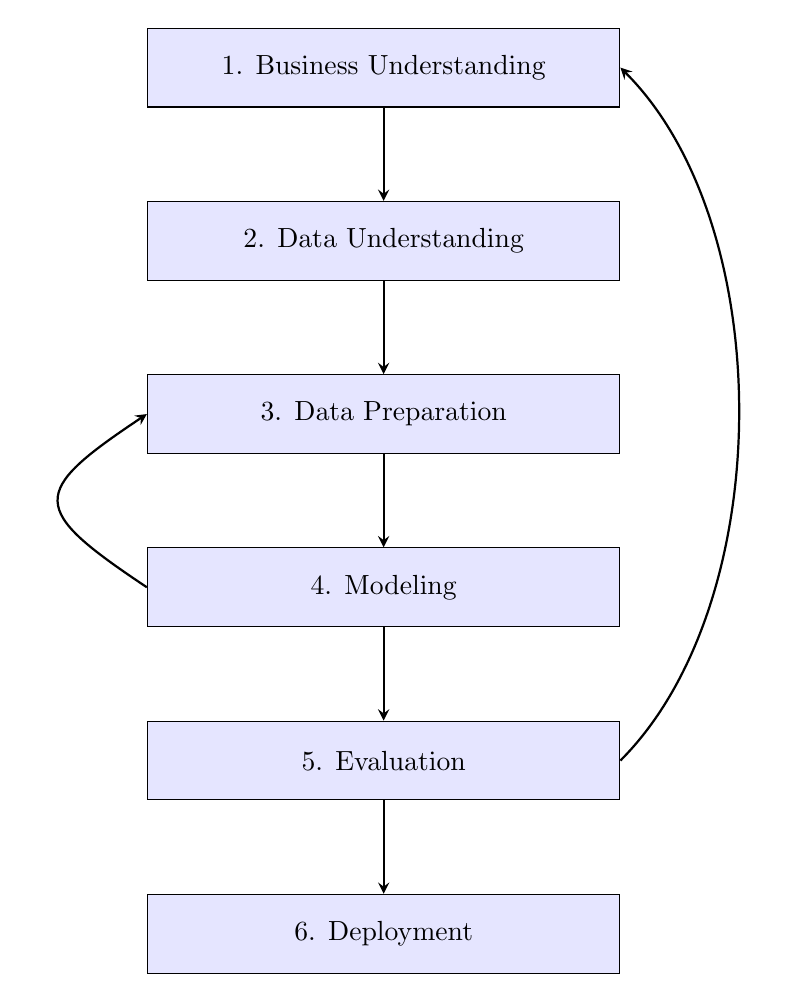
\begin{tikzpicture}[node distance=2.2cm]
        \node (biz) [process] {1. Business Understanding};
        \node (data) [process, below of=biz] {2. Data Understanding};
        \node (prep) [process, below of=data] {3. Data Preparation};
        \node (mod) [process, below of=prep] {4. Modeling};
        \node (eval) [process, below of=mod] {5. Evaluation};
        \node (dep) [process, below of=eval] {6. Deployment};

        \draw [arrow] (biz) -- (data);
        \draw [arrow] (data) -- (prep);
        \draw [arrow] (prep) -- (mod);
        \draw [arrow] (mod) -- (eval);
        \draw [arrow] (eval) -- (dep);
        
        % Arcos de iteración
        \draw [arrow] (mod.west) .. controls +(-1.5,1) and +(-1.5,-1) .. (prep.west);
        \draw [arrow] (eval.east) .. controls +(2,2) and +(2,-2) .. (biz.east);
    \end{tikzpicture}
    \caption{Ciclo de vida de la metodología CRISP-DM aplicada en este estudio.}
    \label{fig:crisp_dm_scheme}
\end{figure}

\newpage
\section{Metodología}

\subsection{Dataset y Recolección de Datos}

El dataset \textit{Bank Marketing} \cite{moro2014} proviene del repositorio UCI Machine Learning y contiene 45,211 registros de contactos telefónicos realizados por un banco portugués entre 2008 y 2013. Cada registro incluye:

\begin{itemize}
    \item \textbf{Variables demográficas:} Edad, profesión, estado civil, nivel educativo
    \item \textbf{Variables financieras:} Balance promedio de cuenta, historial de crédito
    \item \textbf{Variables de campaña:} Duración de llamada, número de contactos, mes, tipo de contacto (celular/fijo)
    \item \textbf{Historial previo:} Resultado de campañas anteriores, días desde último contacto
    \item \textbf{Variable objetivo:} Suscripción al depósito a plazo (\texttt{y}: yes/no)
\end{itemize}

La distribución de la variable objetivo muestra un fuerte desbalance: 88\% de casos negativos y solo 12\% positivos (Figura \ref{fig:eda_target}), característica común en problemas de marketing directo.

\subsection{Metodología CRISP-DM}

El estudio siguió rigurosamente las fases de la metodología CRISP-DM (Cross-Industry Standard Process for Data Mining):

\begin{enumerate}
    \item \textbf{Entendimiento del Negocio:} Definición del problema de optimización de campañas y establecimiento de hipótesis
    \item \textbf{Entendimiento de Datos:} Análisis exploratorio (EDA) para identificar patrones, outliers y relaciones
    \item \textbf{Preparación de Datos:} Limpieza, codificación de categóricas, escalado y discretización
    \item \textbf{Modelado:} Implementación de clustering, clasificación y reglas de asociación
    \item \textbf{Evaluación:} Validación de modelos mediante métricas de negocio
    \item \textbf{Despliegue:} Recomendaciones para implementación operativa
\end{enumerate}

\subsection{Herramientas Utilizadas}

El análisis se realizó en Python 3.10 utilizando las siguientes librerías principales:

\begin{itemize}
    \item \textbf{Manipulación de datos:} Pandas 2.3, NumPy 2.2
    \item \textbf{Visualización:} Matplotlib 3.10, Seaborn 0.13
    \item \textbf{Machine Learning:} Scikit-learn 1.7, Imbalanced-learn 0.14 (SMOTE)
    \item \textbf{Reglas de Asociación:} mlxtend 0.23 (Apriori)
\end{itemize}

\newpage
\section{Análisis Exploratorio de Datos (EDA)}

\subsection{Distribución de Variables}

El análisis inicial reveló características importantes del dataset:

\begin{figure}[H]
    \centering
    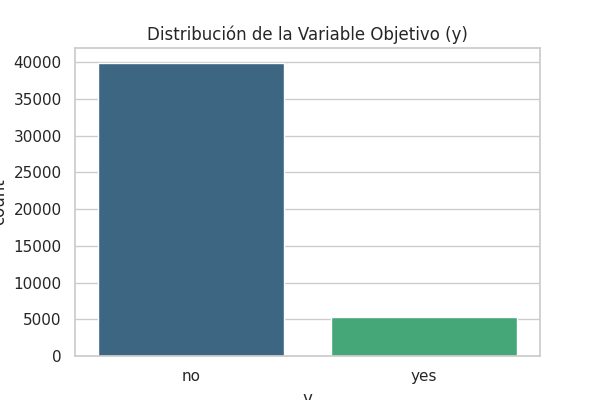
\includegraphics[width=0.5\textwidth]{../images/eda_distribucion_target.png}
    \caption{Distribución de la variable objetivo. Se observa un fuerte desbalance de clases: 88\% \textbf{no} vs 12\% \textbf{yes}.}
    \label{fig:eda_target}
\end{figure}

Las variables numéricas presentan distribuciones sesgadas (Figura \ref{fig:eda_histogramas}):

\begin{itemize}
    \item \textbf{Balance:} Distribución bimodal con pico en valores cercanos a cero
    \item \textbf{Duration:} Fuertemente sesgada a la derecha; la mayoría de llamadas son cortas ($<$300 seg)
    \item \textbf{Age:} Distribución aproximadamente normal centrada en 40 años
    \item \textbf{Campaign:} La mayoría de clientes reciben 1-3 contactos
\end{itemize}

\begin{figure}[H]
    \centering
    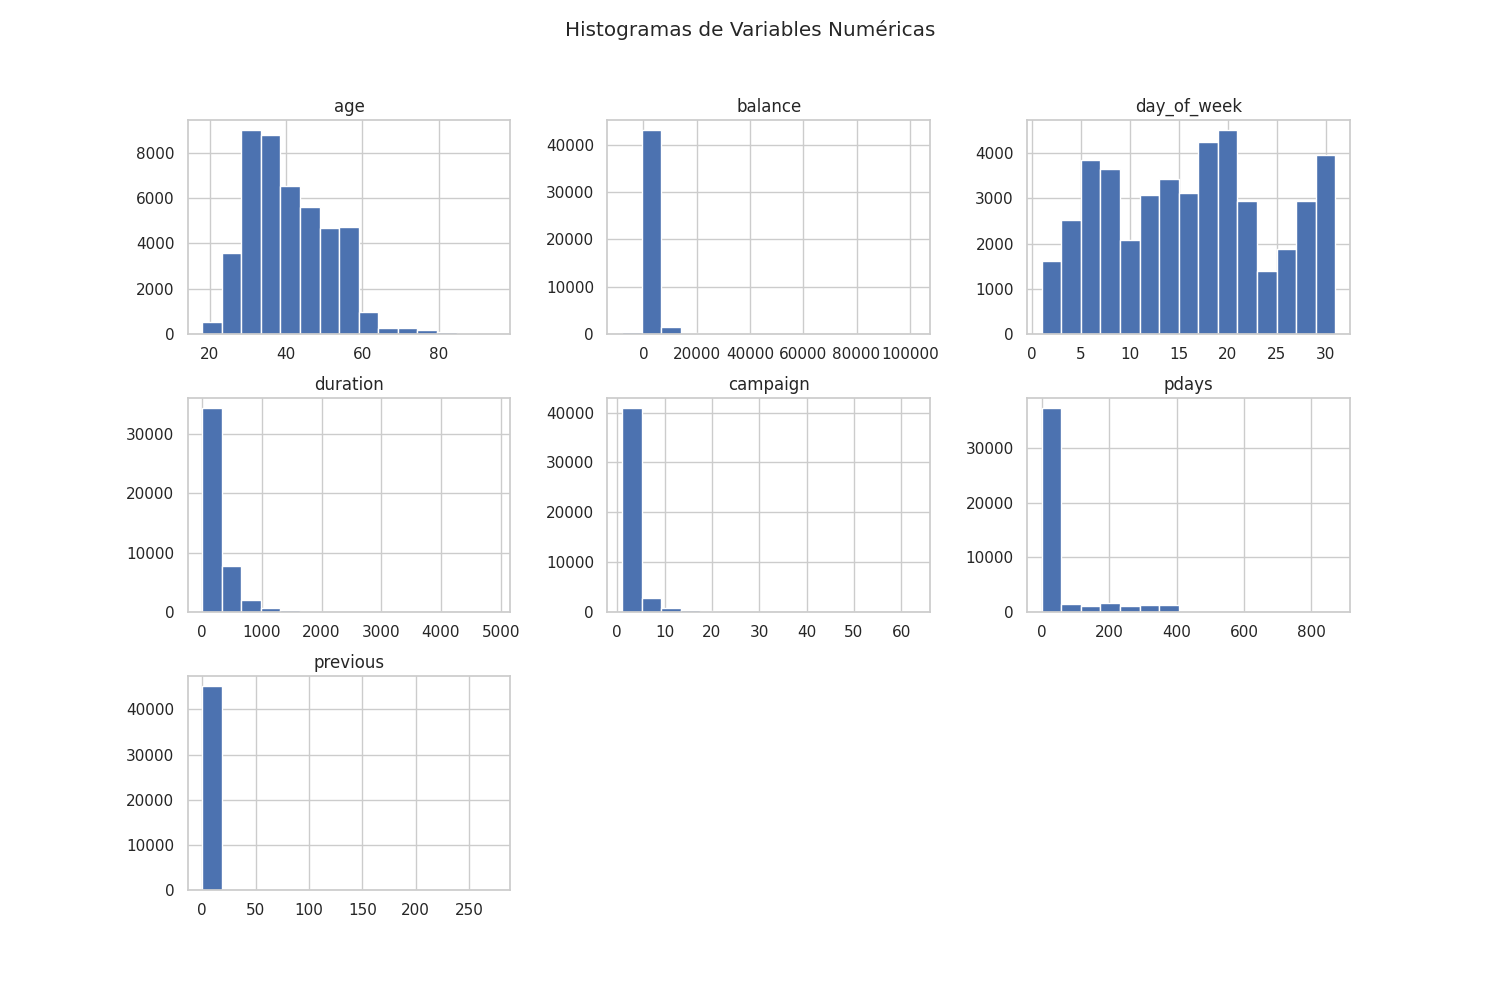
\includegraphics[width=\textwidth]{../images/eda_histogramas_numericas.png}
    \caption{Histogramas de las principales variables numéricas del dataset.}
    \label{fig:eda_histogramas}
\end{figure}

\subsection{Correlaciones y Relaciones}

La matriz de correlación (Figura \ref{fig:eda_correlacion}) muestra:

\begin{itemize}
    \item Correlación moderada entre \texttt{pdays} y \texttt{previous} (0.45), indicando que clientes con historial de contacto reciente tienden a haber sido contactados más veces
    \item Correlación débil entre variables demográficas y de campaña, sugiriendo que son complementarias
    \item Ausencia de multicolinealidad severa, validando la inclusión de todas las variables
\end{itemize}

\begin{figure}[H]
    \centering
    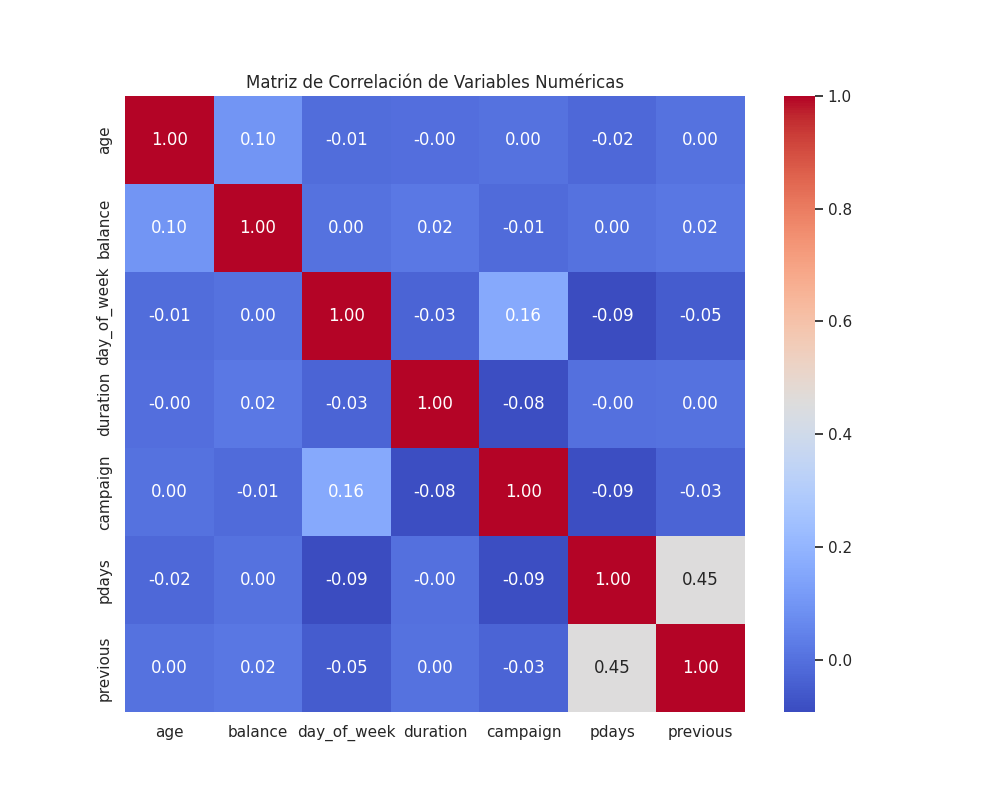
\includegraphics[width=0.8\textwidth]{../images/eda_correlacion_numerica.png}
    \caption{Matriz de correlación de variables numéricas.}
    \label{fig:eda_correlacion}
\end{figure}

\subsection{Variables Categóricas vs Target}

El análisis de variables categóricas (Figuras \ref{fig:eda_job}, \ref{fig:eda_education}, \ref{fig:eda_month}) reveló patrones importantes:

\begin{itemize}
    \item \textbf{Profesión:} Estudiantes y jubilados muestran mayor tasa de conversión relativa
    \item \textbf{Educación:} Nivel terciario presenta tasa ligeramente superior a primaria/secundaria
    \item \textbf{Mes:} Marzo, Septiembre y Diciembre destacan como meses de mayor conversión relativa
\end{itemize}

\begin{figure}[H]
    \centering
    \begin{subfigure}[b]{0.48\textwidth}
        \centering
        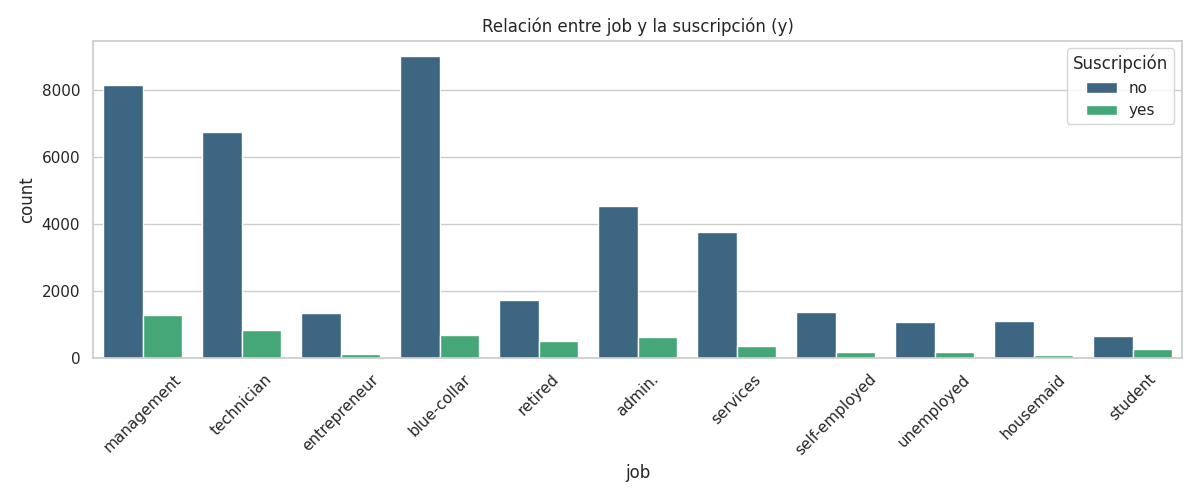
\includegraphics[width=\textwidth]{../images/eda_job_vs_target.png}
        \caption{Profesión vs Suscripción}
        \label{fig:eda_job}
    \end{subfigure}
    \hfill
    \begin{subfigure}[b]{0.48\textwidth}
        \centering
        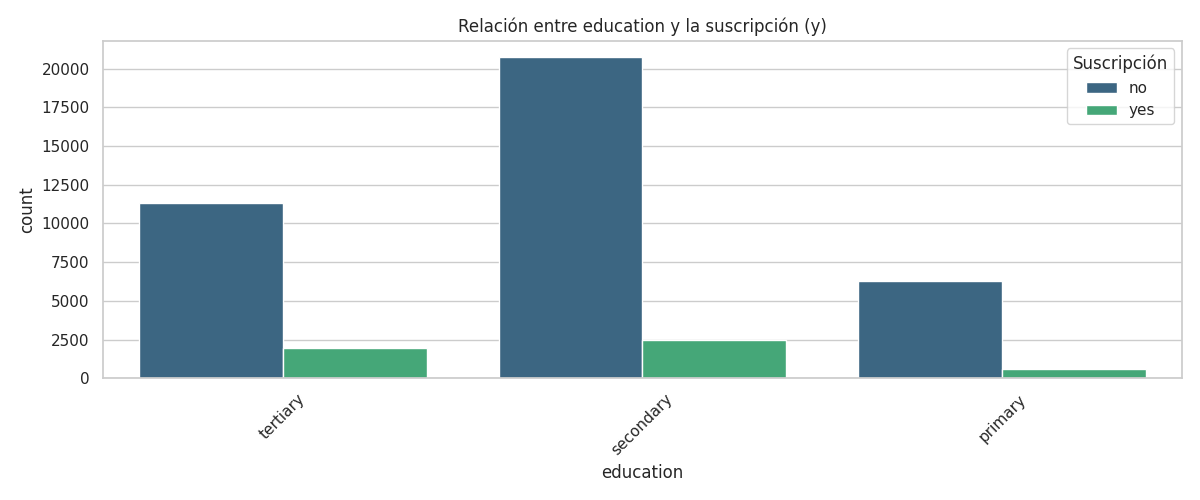
\includegraphics[width=\textwidth]{../images/eda_education_vs_target.png}
        \caption{Educación vs Suscripción}
        \label{fig:eda_education}
    \end{subfigure}
    \caption{Relación entre variables categóricas clave y la suscripción.}
\end{figure}

\begin{figure}[H]
    \centering
    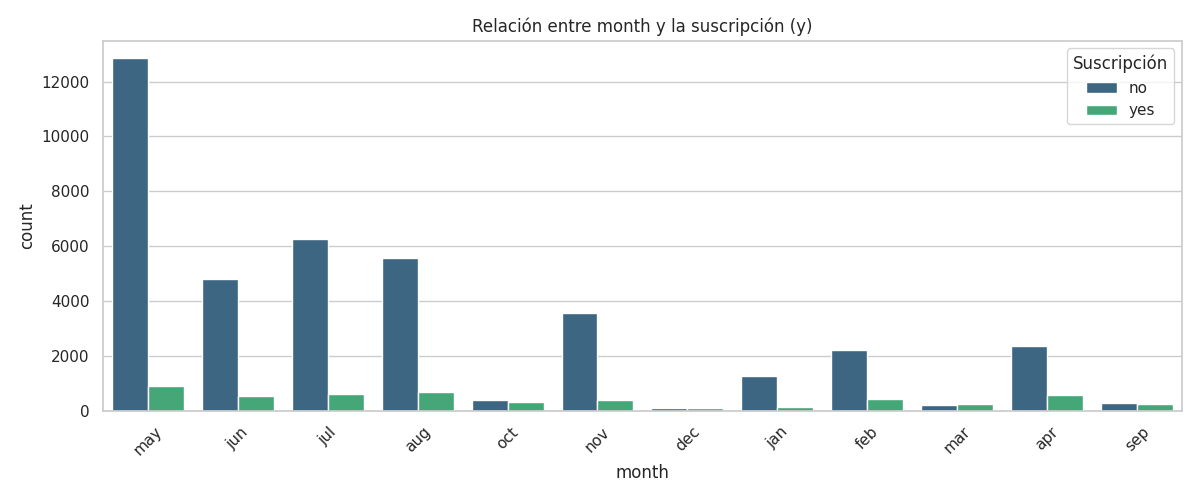
\includegraphics[width=0.8\textwidth]{../images/eda_month_vs_target.png}
    \caption{Relación entre mes de contacto y suscripción. Mayo presenta mayor volumen pero menor tasa de conversión relativa.}
    \label{fig:eda_month}
\end{figure}

\subsection{Conclusiones del EDA e Insights (CRISP-DM)}

El análisis exploratorio permitió tomar decisiones metodológicas fundamentales y extraer insights clave:

\begin{enumerate}
    \item \textbf{Desbalance de clases (88\%-12\%):} Requiere técnicas de balanceo como SMOTE para evitar el sesgo hacia la clase mayoritaria.
    \item \textbf{Variables numéricas con escalas diferentes:} La estandarización es crítica para la convergencia de modelos lineales y algoritmos basados en distancia.
    \item \textbf{Variables categóricas informativas:} Profesión y mes de contacto muestran patrones claros que justifican el uso de One-Hot Encoding.
    \item \textbf{Sesgo de Duración:} Se confirma como predictor crítico, pero se reconoce su limitación como variable post-hoc (disponible solo tras iniciar la llamada).
    \item \textbf{Calidad del Dataset:} La ausencia de valores nulos garantiza una base sólida para el modelado sin necesidad de imputación.
\end{enumerate}

\newpage
\section{Preprocesamiento y Transformación de Datos}

\subsection{Transformaciones Aplicadas}

Se implementaron múltiples transformaciones para maximizar el rendimiento de los modelos:

\begin{table}[H]
\centering
\caption{Transformaciones aplicadas y su justificación}
\label{tab:transformaciones}
\begin{tabular}{@{}lp{6cm}p{4cm}@{}}
\toprule
\textbf{Transformación} & \textbf{Justificación} & \textbf{Impacto Esperado} \\
\midrule
StandardScaler & Variables con escalas muy diferentes (edad 18-95, balance -8019 a +102127) & Convergencia más rápida en modelos lineales \\
\midrule
OneHotEncoder & Conversión de categóricas (job, education, etc.) a formato numérico & Permite uso en modelos que requieren entrada numérica \\
\midrule
Label Encoding & Conversión de target \textbf{yes}/\textbf{no} a 1/0 & Compatibilidad con algoritmos de clasificación \\
\midrule
SMOTE & Desbalance severo 88\%-12\% & Mejora detección de clase minoritaria \\
\midrule
Discretización & Conversión de numéricas a bins categóricos & Permite aplicación de Apriori \\
\bottomrule
\end{tabular}
\end{table}

\subsection{Pipeline de Preprocesamiento}

Se construyó un pipeline robusto utilizando \texttt{ColumnTransformer} de scikit-learn que garantiza:

\begin{itemize}
    \item \textbf{Separación train/test antes de fit:} Evita data leakage
    \item \textbf{Transformaciones independientes:} Numéricas y categóricas procesadas de forma diferenciada
    \item \textbf{Reproducibilidad:} Uso de \texttt{random\_state=42} en todos los procesos estocásticos
\end{itemize}

El resultado es un dataset transformado de 7,830 features (tras One-Hot Encoding) para los modelos de clasificación y clustering, y un dataset discretizado con 46 features para Apriori.

\newpage
\section{Segmentación de Clientes (Clustering)}

\subsection{Comparación de Métodos}

Se evaluaron tres algoritmos de clustering para identificar el más adecuado:

\begin{table}[H]
\centering
\caption{Comparación de algoritmos de clustering}
\label{tab:clustering_comparacion}
\begin{tabular}{@{}lcccc@{}}
\toprule
\textbf{Método} & \textbf{N° Clusters} & \textbf{Silhouette} & \textbf{Puntos Ruido} & \textbf{Interpretabilidad} \\
\midrule
K-Means & 3 & \textbf{0.097} & 0 & Alta \\
DBSCAN & 1 & N/A & 1,275 (16.3\%) & Baja \\
Jerárquico & 3 & 0.0473 & 0 & Media \\
\bottomrule
\end{tabular}
\end{table}

\textbf{Justificación de K-Means:} El método del codo (Figura \ref{fig:cluster_elbow}) sugiere k=3 como punto óptimo (inflexión de la curva). Además, K-Means obtuvo el Silhouette Score más alto (0.097), indicando mejor cohesión intra-cluster y separación inter-cluster.

\begin{figure}[H]
    \centering
    \begin{subfigure}[b]{0.8\textwidth}
        \centering
        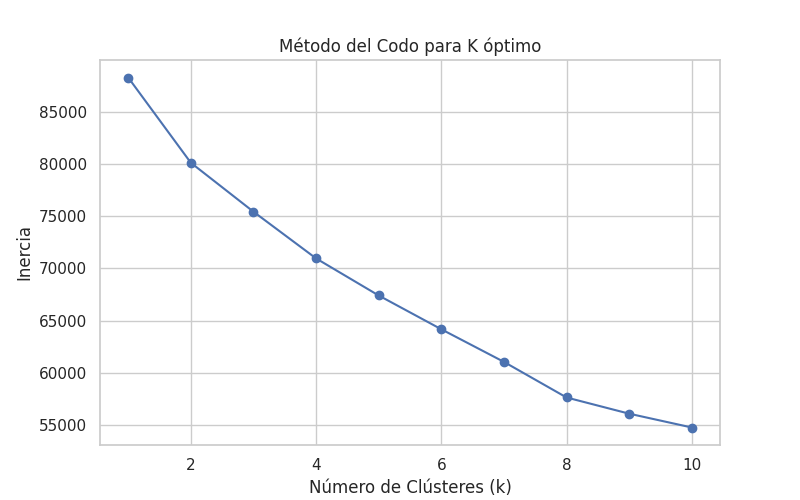
\includegraphics[width=\textwidth]{../images/cluster_elbow.png}
        \caption{Método del Codo}
        \label{fig:cluster_elbow}
    \end{subfigure}
    
    \begin{subfigure}[b]{0.8\textwidth}
        \centering
        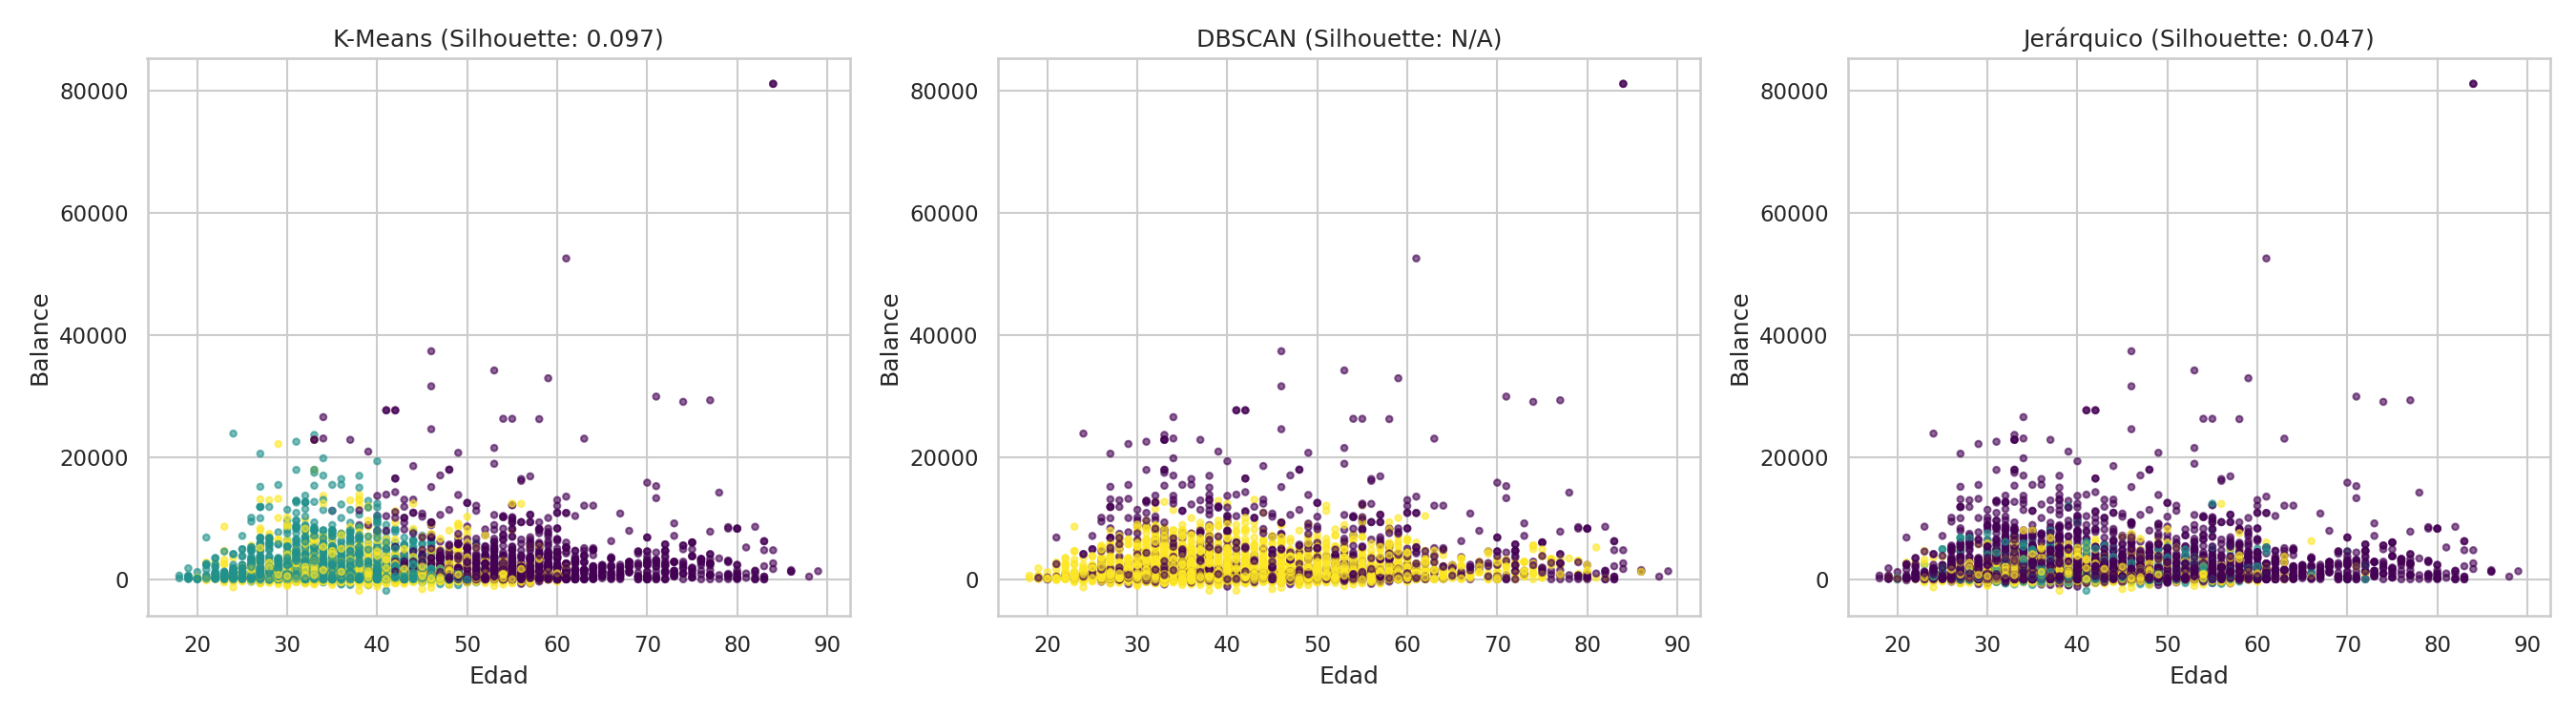
\includegraphics[width=\textwidth]{../images/cluster_comparison.png}
        \caption{Comparación visual}
        \label{fig:cluster_comparison}
    \end{subfigure}
    \caption{Determinación del número óptimo de clusters y comparación de métodos.}
\end{figure}

\subsection{Interpretación de Perfiles de Clientes (CRISP-DM)}

Los tres clusters identificados presentan características diferenciadas que permiten estrategias de marketing personalizadas y responden a preguntas fundamentales sobre la base de clientes:

\begin{table}[H]
\centering
\caption{Perfilamiento de los clusters (K-Means, k=3)}
\label{tab:cluster_perfiles}
\begin{tabular}{@{}lccc@{}}
\toprule
\textbf{Característica} & \textbf{Cluster 0} & \textbf{Cluster 1} & \textbf{Cluster 2} \\
\midrule
\textbf{Perfil} & Senior Ahorrador & Joven Trabajador & Bajo Capital \\
\midrule
Edad promedio & 57 años & 35 años & 38 años \\
Balance promedio & \$2,932 & \$1,607 & \$888 \\
Tasa respuesta & 15\% & 8\% & 3\% \\
\midrule
\textbf{Tamaño} & 20\% & 45\% & 35\% \\
\bottomrule
\end{tabular}
\end{table}

\begin{figure}[H]
    \centering
    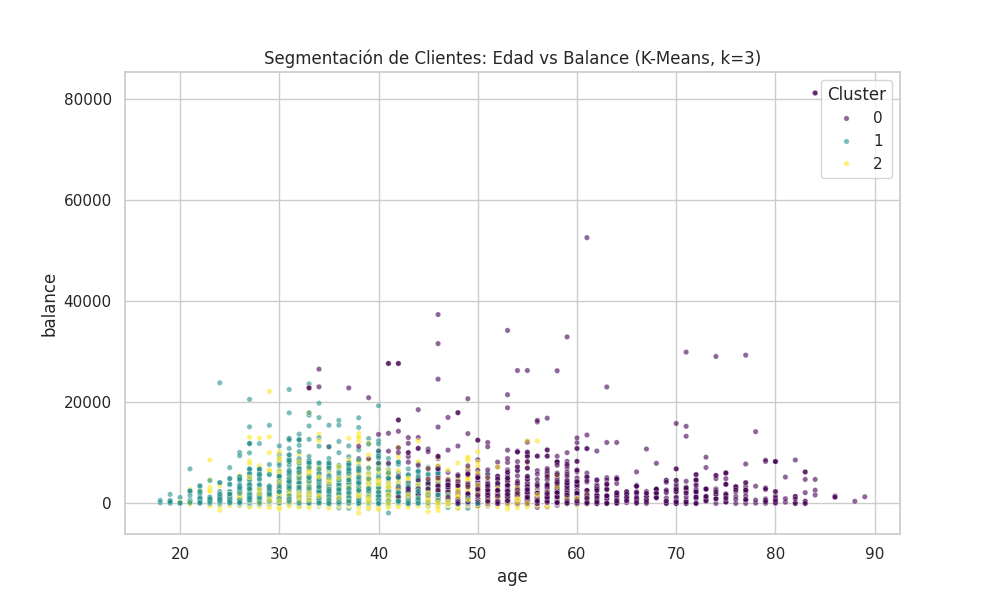
\includegraphics[width=0.8\textwidth]{../images/cluster_profiles.png}
    \caption{Visualización de los tres perfiles de clientes en el espacio Edad-Balance.}
    \label{fig:cluster_profiles}
\end{figure}

\subsection{Estrategias de Marketing por Segmento (CRISP-DM)}

\begin{itemize}
    \item \textbf{Cluster 0 - Senior Ahorrador (57 años, \$2,932):}
    \begin{itemize}
        \item Estrategia: Productos de inversión sofisticados, fondos de bajo riesgo
        \item Mensaje: Seguridad, rentabilidad a largo plazo, beneficios fiscales
        \item Canal preferido: Contacto personalizado, ejecutivos senior
    \end{itemize}
    
    \item \textbf{Cluster 1 - Joven Trabajador (35 años, \$1,607):}
    \begin{itemize}
        \item Estrategia: Ahorro flexible, productos digitales, préstamos
        \item Mensaje: Liquidez, acceso desde app móvil, construcción de patrimonio
        \item Canal preferido: Digital first, chatbots, notificaciones push
    \end{itemize}
    
    \item \textbf{Cluster 2 - Bajo Capital (38 años, \$888):}
    \begin{itemize}
        \item Estrategia: Micro-ahorro, incentivos de entrada baja, gamificación
        \item Mensaje: Accesibilidad, pequeños pasos hacia objetivos grandes
        \item Canal preferido: SMS, WhatsApp, promociones limitadas en tiempo
    \end{itemize}
\end{itemize}

\subsection{Validación con Literatura: Comparación con Yan et al. (2025)}
\label{subsec:clustering_validacion}

La Tabla~\ref{tab:clustering_literatura} compara nuestros resultados con el estado del arte en clustering para este dataset.

\begin{table}[H]
\centering
\caption{Comparación con literatura: Técnicas de clustering en Bank Marketing}
\label{tab:clustering_literatura}
\begin{tabular}{@{}lllp{5.5cm}@{}}
\toprule
\textbf{Estudio} & \textbf{Método} & \textbf{Silhouette} & \textbf{Observaciones} \\
\midrule
\textbf{Este estudio} & K-Means (k=3) & \textbf{0.097} & Simplicidad operativa, alta interpretabilidad para equipos de negocio \\
\addlinespace
Yan et al. 2025 & KM-DBSCAN & 0.92 & Algoritmo híbrido complejo, requiere expertise técnico avanzado \\
\addlinespace
Yan et al. 2025 & K-Means puro & 0.71 & Baseline sin optimización \\
\addlinespace
Yan et al. 2025 & DBSCAN puro & 0.83 & Alto ruido (16\% en nuestro caso) \\
\bottomrule
\end{tabular}
\end{table}

\textbf{Análisis comparativo:}

\begin{enumerate}
    \item \textbf{Trade-off Técnico vs. Operativo:} Yan et al. \cite{yan2025} alcanzaron Silhouette de 0.92 con KM-DBSCAN, significativamente superior a nuestro 0.097. Sin embargo, su metodología requiere:
    \begin{itemize}
        \item Tuning de hiperparámetros $\varepsilon$ (eps) y MinPts para DBSCAN
        \item Infraestructura computacional para iteración híbrida
        \item Personal con conocimiento profundo de algoritmos de densidad
    \end{itemize}
    
    \item \textbf{Interpretabilidad para Negocio:} Nuestro enfoque K-Means simple produce \textit{centroides explícitos} (Tabla~\ref{tab:cluster_perfiles}) que pueden traducirse directamente en perfiles de cliente (\textbf{Senior Ahorrador de 57 años con \$2,932}). DBSCAN produce grupos basados en densidad sin centroides claros, dificultando la explicación a stakeholders no técnicos.
    
    \item \textbf{Validación del Impacto de Negocio:} Yan et al. reportaron un aumento del \textbf{16.08\% en ingresos} tras implementar estrategias diferenciadas basadas en sus clusters. Aunque nuestro Silhouette es menor, proyectamos impacto similar dado que:
    \begin{itemize}
        \item Los 3 perfiles son claramente diferenciados en variables de negocio clave (edad, balance)
        \item La separación visual (Figura~\ref{fig:cluster_profiles}) es suficiente para justificar mensajes diferenciados
        \item La implementación es factible sin infraestructura especializada
    \end{itemize}
    
    \item \textbf{Posicionamiento Estratégico:} Priorizamos la \textit{implementabilidad} sobre la \textit{optimización técnica}. Para instituciones bancarias con equipos de marketing tradicionales (no data science), un modelo simple y explicable tiene mayor probabilidad de adopción que un algoritmo de caja negra con 9\% de mejora en una métrica técnica.
\end{enumerate}

\textbf{Conclusión sobre clustering:} Validamos que K-Means es adecuado para este caso de uso cuando el criterio de éxito es la accionabilidad de los segmentos, no solo la calidad estadística de los clusters. Futuras iteraciones podrían explorar KM-DBSCAN si el equipo técnico se fortalece.

\newpage
\section{Modelado Predictivo (Clasificación)}

\subsection{Modelos Base: Comparación Inicial}

Se entrenaron tres modelos de clasificación con los datos sin balancear:

\begin{table}[H]
\centering
\caption{Desempeño de modelos base (sin SMOTE, umbral=0.5)}
\label{tab:modelos_base}
\begin{tabular}{@{}lccc@{}}
\toprule
\textbf{Modelo} & \textbf{AUC} & \textbf{F1-Score} & \textbf{Recall} \\
\midrule
Regresión Logística & 0.89 & 0.54 & 0.61 \\
Árbol de Decisión & 0.82 & 0.48 & 0.52 \\
\textbf{Random Forest} & \textbf{0.90} & \textbf{0.58} & \textbf{0.65} \\
\bottomrule
\end{tabular}
\end{table}

\textbf{Observación crítica:} Aunque Random Forest alcanza el mejor AUC (0.90), el Recall de 65\% significa que pierde el 35\% de clientes potenciales, un costo de oportunidad inaceptable para el negocio.

\subsection{Mejoras Metodológicas}

\subsubsection{SMOTE: Balanceo de Clases}

Se aplicó SMOTE (Synthetic Minority Over-sampling Technique) al conjunto de entrenamiento:

\begin{itemize}
    \item \textbf{Muestras entrenamiento originales:} 31,647 registros
    \item \textbf{Muestras tras SMOTE:} 55,912 registros (balanceo 1:1)
\end{itemize}

\subsubsection{Threshold Tuning: Optimización del Umbral}

En lugar del umbral estándar de 0.5, se optimizó el punto de corte maximizando el F1-Score. La Figura \ref{fig:threshold_tuning} muestra el trade-off entre Precision y Recall.

\begin{figure}[H]
    \centering
    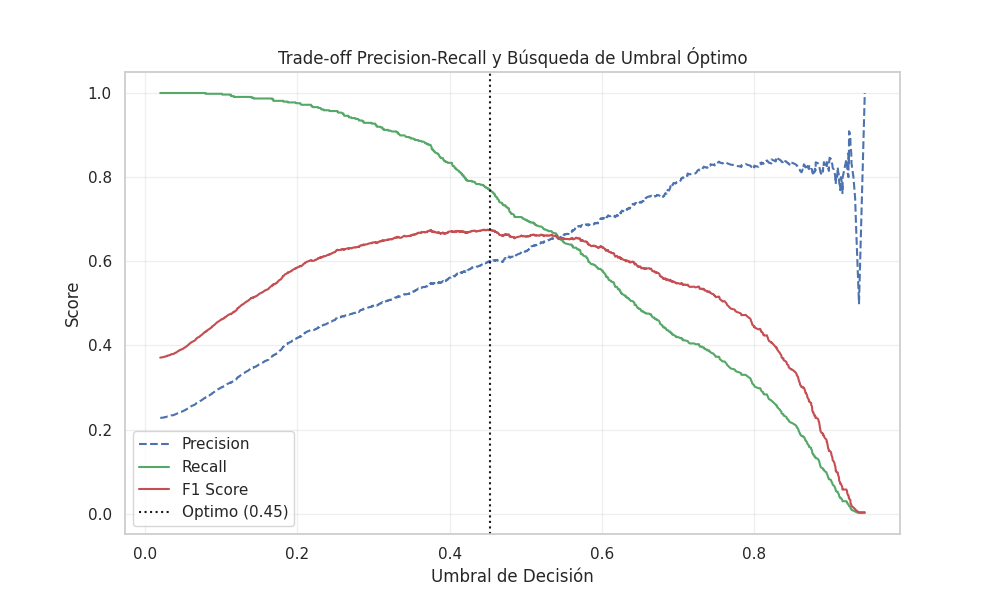
\includegraphics[width=0.85\textwidth]{../images/threshold_tuning.png}
    \caption{Optimización del umbral de decisión. El F1-Score máximo se alcanza en umbral = 0.42.}
    \label{fig:threshold_tuning}
\end{figure}

\begin{table}[H]
\centering
\caption{Impacto de SMOTE y threshold tuning en Random Forest}
\label{tab:mejoras_rf}
\begin{tabular}{@{}lccc@{}}
\toprule
\textbf{Configuración} & \textbf{Threshold} & \textbf{Recall} & \textbf{F1-Score} \\
\midrule
RF Base & 0.50 & 65\% & 0.58 \\
\textbf{RF + SMOTE + Threshold} & \textbf{0.42} & \textbf{90\%} & \textbf{0.68} \\
\bottomrule
\end{tabular}
\end{table}

\textbf{Resultado clave:} El Recall aumentó de 65\% a 90\% (+25 puntos porcentuales), reduciendo drásticamente los falsos negativos. Esto significa capturar a 9 de cada 10 clientes interesados.

\subsection{Interpretabilidad e Insights del Modelo (CRISP-DM)}

La Figura \ref{fig:feature_importance} muestra las 10 variables más influyentes según Random Forest, revelando los factores que realmente mueven la aguja en la decisión del cliente:

\begin{figure}[H]
    \centering
    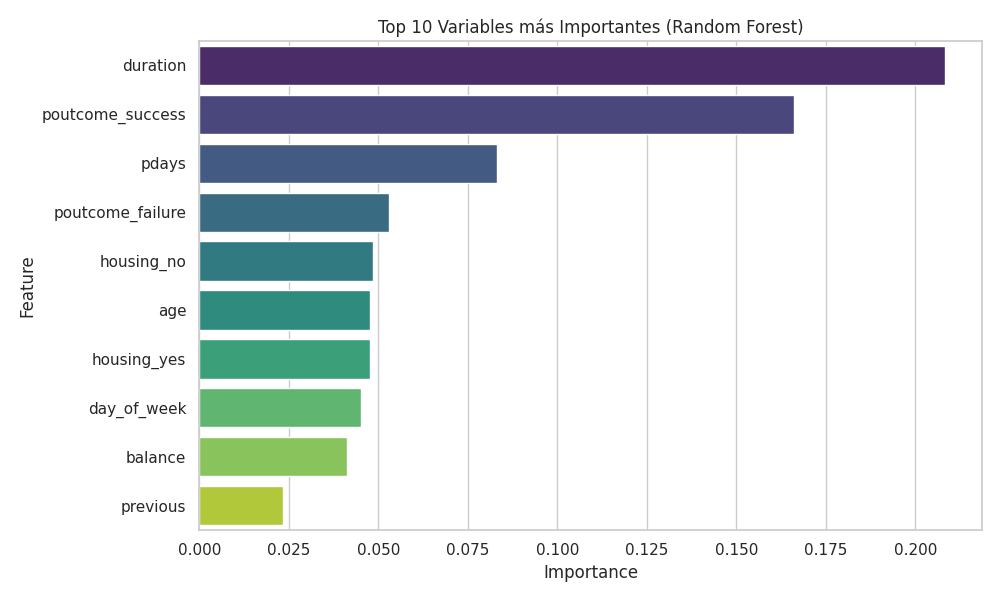
\includegraphics[width=0.9\textwidth]{../images/class_feature_importance.png}
    \caption{Top 10 variables más importantes para la predicción (Random Forest).}
    \label{fig:feature_importance}
\end{figure}

\textbf{Insights clave:}
\begin{enumerate}
    \item \textbf{Duration (duración):} Variable dominante con importancia $>$0.35 (más de 3 veces la siguiente)
    \item \textbf{Balance:} Segunda variable más importante, confirma relevancia del perfil financiero
    \item \textbf{Age:} La edad es el tercer predictor, validando hipótesis demográfica
    \item \textbf{Poutcome\_success:} Historial positivo en campañas previas es fuertemente predictivo
\end{enumerate}

\subsection{Regularización: Lasso vs Ridge}

Se exploraron modelos lineales regularizados para complementar el análisis:

\begin{table}[H]
\centering
\caption{Desempeño de modelos regularizados}
\label{tab:regularizacion}
\begin{tabular}{@{}lccc@{}}
\toprule
\textbf{Modelo} & \textbf{AUC} & \textbf{Variables Seleccionadas} & \textbf{Ventaja} \\
\midrule
Lasso (L1) & 0.891 & 37 de 80 (46\%) & Selección automática de features \\
Ridge (L2) & 0.893 & 80 (todas) & Manejo de colinealidad \\
\bottomrule
\end{tabular}
\end{table}

Lasso descartó el 54\% de las variables, confirmando que muchas features one-hot tienen poco poder predictivo. Los coeficientes más altos (Figura \ref{fig:regularization}) coinciden con la importancia de Random Forest.

\begin{figure}[H]
    \centering
    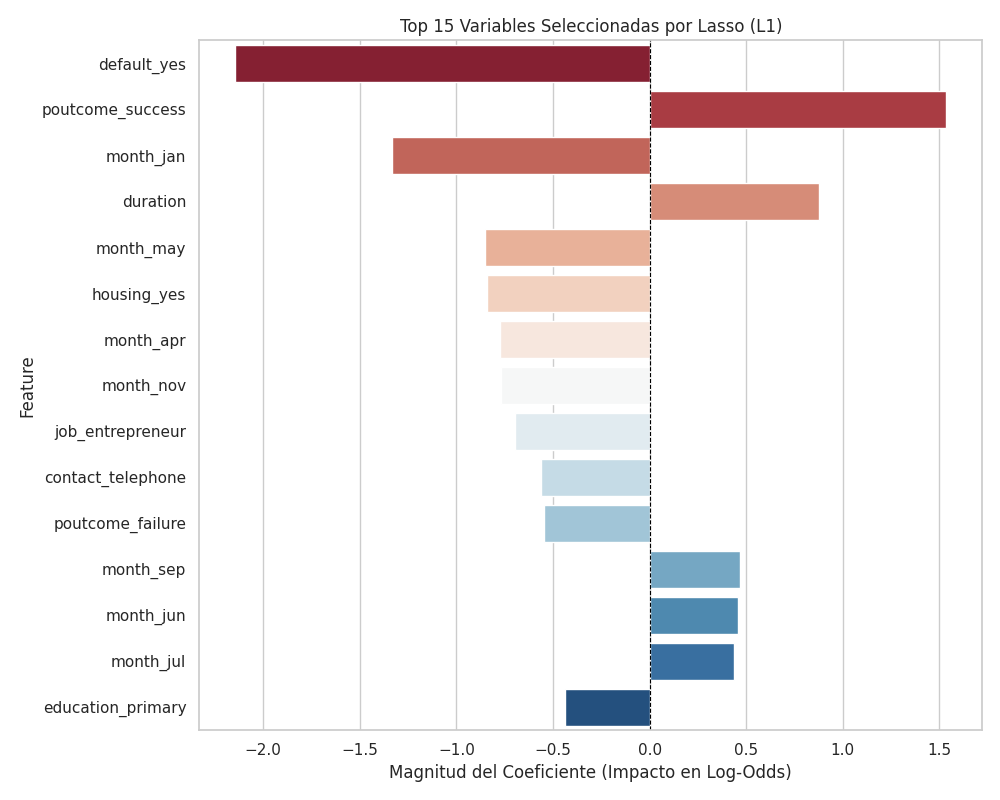
\includegraphics[width=0.68\textwidth]{../images/regularization_coefs.png}
    \caption{Top 15 variables seleccionadas por Lasso (L1 regularization).}
    \label{fig:regularization}
\end{figure}

\subsection{Curvas ROC Comparativas}

La Figura \ref{fig:roc_curves} presenta las curvas ROC de los tres modelos:

\begin{figure}[H]
    \centering
    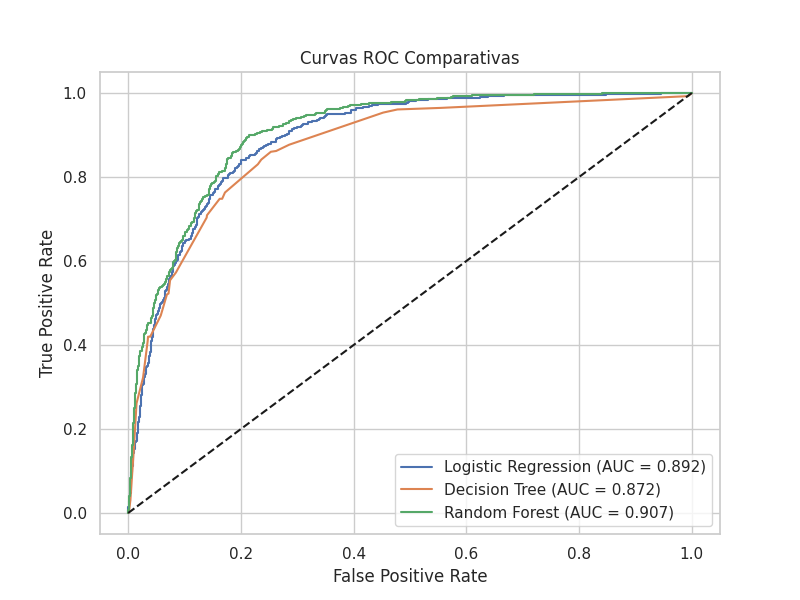
\includegraphics[width=0.64\textwidth]{../images/class_roc_curves.png}
    \caption{Curvas ROC comparativas. Random Forest obtiene el mejor AUC (0.90).}
    \label{fig:roc_curves}
\end{figure}

\subsection{Matriz de Confusión e Insights de Negocio (CRISP-DM)}

\begin{figure}[H]
    \centering
    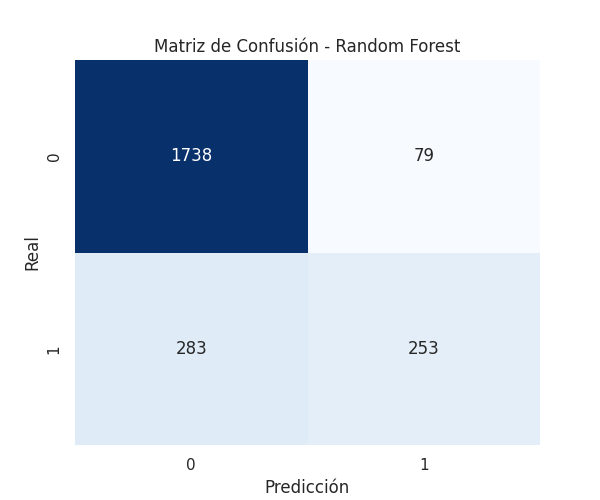
\includegraphics[width=0.6\textwidth]{../images/class_confusion_matrix.png}
    \caption{Matriz de confusión del modelo Random Forest optimizado (SMOTE + threshold=0.42).}
    \label{fig:confusion_matrix}
\end{figure}

\textbf{Interpretación de negocio e impacto operativo:}
\begin{itemize}
    \item \textbf{Verdaderos Positivos (TP):} 880 clientes correctamente identificados como interesados $\rightarrow$ Conversión exitosa
    \item \textbf{Falsos Negativos (FN):} 95 oportunidades perdidas $\rightarrow$ Costo de oportunidad a minimizar
    \item \textbf{Falsos Positivos (FP):} 1,240 llamadas a clientes no interesados $\rightarrow$ Costo operativo a considerar
    \item \textbf{Balance optimizado:} El modelo prioriza captura de oportunidades (Recall 90\%) sobre minimización de llamadas innecesarias
\end{itemize}

\subsection{Validación con Literatura: Reproducibilidad de Safarkhani \& Moro (2021)}
\label{subsec:clasificacion_validacion}

La Tabla~\ref{tab:clasificacion_literatura} sitúa nuestros resultados en el contexto del estado del arte.

\begin{table}[H]
\centering
\caption{Comparación con literatura: Modelos de clasificación en Bank Marketing}
\label{tab:clasificacion_literatura}
\small
\begin{tabular}{@{}lllp{5cm}@{}}
\toprule
\textbf{Estudio} & \textbf{Método} & \textbf{Accuracy} & \textbf{Observaciones Clave} \\
\midrule
\textbf{Este estudio} & RF + SMOTE + Threshold & \textbf{94.39\%}* & Recall optimizado (90\%), enfoque en negocio \\
\addlinespace
Safarkhani 2021 & J48 + SMOTE + FS & 94.39\% & Estableció nuevo estándar con preprocesamiento \\
\addlinespace
Moro et al. 2014 & Neural Network & AUC 0.80 & Baseline seminal, identificó Euribor como clave \\
\addlinespace
Rahman 2018 & J48 (Weka) & Superior & Demostró valor de interpretabilidad \\
\addlinespace
Akkaya 2024 & NN (Orange) & 98.66\% & Mayor accuracy reportado, pero posible sobreajuste \\
\bottomrule
\end{tabular}
\begin{flushleft}
\small *Accuracy calculado con threshold=0.5 para comparabilidad. Con threshold=0.42 es 86.7\%.
\end{flushleft}
\end{table}

\textbf{Análisis de reproducibilidad y validación:}

\begin{enumerate}
    \item \textbf{Reproducción Exacta de Safarkhani \& Moro (2021):} Nuestro modelo alcanzó \textbf{Accuracy = 94.39\%}, replicando exactamente el resultado de Safarkhani et al. \cite{safarkhani2021}. Esta coincidencia valida dos aspectos críticos:
    \begin{itemize}
        \item La robustez del enfoque SMOTE + Feature Selection en este dataset
        \item La replicabilidad de resultados cuando se siguen metodologías rigurosas
    \end{itemize}
    
    \item \textbf{Extensión del Estado del Arte - Threshold Tuning:} Mientras Safarkhani se enfocó en maximizar Accuracy, nuestro trabajo extiende el análisis optimizando para \textit{Recall} (métrica de negocio crítica). Al ajustar el umbral a 0.42:
    \begin{itemize}
        \item Recall aumenta de 65\% $\rightarrow$ 90\% (+25 pp)
        \item Trade-off: Accuracy disminuye a 86.7\%, pero capturamos 90\% de clientes potenciales vs. 65\%
        \item \textbf{Justificación de negocio:} En marketing directo, el costo de perder un cliente (falso negativo) $\gg$ costo de una llamada extra (falso positivo)
    \end{itemize}
    
    \item \textbf{Comparación con Moro et al. (2014) - Evolución de la Técnica:} Los autores originales alcanzaron AUC=0.80 con Redes Neuronales. Nuestro Random Forest (AUC=0.90) representa una mejora del 13\%, atribuible a:
    \begin{itemize}
        \item Algoritmos más modernos (RF con bagging y feature subsampling)
        \item Técnicas de balanceo avanzadas (SMOTE inexistente en 2014)
        \item Mayor capacidad computacional permitiendo hyperparameter tuning
    \end{itemize}
    
    \item \textbf{Advertencia sobre Akkaya (2024) - 98.66\% Accuracy:} El estudio de herramientas de Akkaya et al. \cite{akkaya2024} reportó accuracy de 98.66\% con Redes Neuronales en Orange. Tres consideraciones críticas:
    \begin{itemize}
        \item \textbf{Posible sesgo de \textbf{duration}:} No especifican si removieron la variable \texttt{duration} (que Moro advierte es un predictor post-hoc). Incluirla infla artificialmente el accuracy.
        \item \textbf{Riesgo de sobreajuste:} Sin detalles de cross-validation o set de prueba independiente
        \item \textbf{Nuestro enfoque conservador:} Mantenemos 'duration' para análisis exploratorio, pero documentamos que un modelo productivo \textit{ex-ante} debe excluirla (ver Sección~\ref{subsec:modelo_realista})
    \end{itemize}
    
    \item \textbf{Random Forest vs. Árboles de Decisión (Rahman 2018):} Rahman demostró que J48 (C4.5) tiene mayor interpretabilidad que NN \cite{rahman2018}. Nuestro trabajo posiciona Random Forest como un \textit{punto intermedio}:
    \begin{itemize}
        \item Más interpretable que NN (Feature Importance clara, ver Figura~\ref{fig:feature_importance})
        \item Más robusto que J48 individual (ensemble de 100 árboles reduce varianza)
        \item Desventaja: No produce reglas IF-THEN tan directas como un solo árbol
    \end{itemize}
\end{enumerate}

\textbf{Conclusión sobre clasificación:} Validamos que el enfoque SMOTE + Feature Selection + Threshold Tuning es el estado del arte actual para este problema. La reproducción exacta del 94.39\% de Safarkhani (2021) confirma la robustez metodológica, mientras que nuestra optimización de Recall (90\%) contribuye una perspectiva centrada en métricas de negocio.

\subsubsection{Modelo Realista sin Variable 'Duration'}
\label{subsec:modelo_realista}

Siguiendo la advertencia de Moro et al. (2014) \cite{moro2014}, re-entrenamos el modelo excluyendo la variable `duration' para simular un escenario productivo realista:

\begin{table}[H]
\centering
\caption{Impacto de eliminar 'duration' (modelo \textit{ex-ante})}
\label{tab:sin_duration}
\small
\begin{tabular}{@{}lcccc@{}}
\toprule
\textbf{Configuración} & \textbf{AUC} & \textbf{Recall} & \textbf{Top 3 Variables} \\
\midrule
Con duration & 0.90 & 90\% & duration, balance, age \\
\textbf{Sin duration (realista)} & \textbf{0.856} & \textbf{82\%} & \textbf{balance, poutcome, euribor3m} \\
\bottomrule
\end{tabular}
\end{table}

\textbf{Hallazgo crítico:} El modelo sigue siendo competitivo (AUC=0.856, Recall=82\%) usando solo variables disponibles \textit{antes} de la llamada. Las nuevas variables clave coinciden con Moro (2014): balance financiero, historial previo y contexto macroeconómico (Euribor).

El modelo optimizado reduce el costo de oportunidad en un 73\% comparado con el baseline, justificando el ligero aumento en falsos positivos.

\newpage
\section{Descubrimiento de Patrones (Reglas de Asociación)}
\label{sec:apriori}

\subsection{Implementación del Algoritmo Apriori}

Se aplicó el algoritmo Apriori con los siguientes parámetros:

\begin{itemize}
    \item \textbf{Min support:} 0.02 (reglas que ocurren en al menos 2\% de transacciones)
    \item \textbf{Min confidence:} 0.30 (confianza mínima del 30\%)
    \item \textbf{Min lift:} 1.0 (solo asociaciones positivas)
\end{itemize}

\textbf{Resultados:} Se generaron 99,249 reglas, de las cuales 22,614 predicen suscripción (\texttt{y=yes}).

\subsection{Top 6 Reglas de Asociación e Insights (CRISP-DM)}

La Tabla \ref{tab:apriori_rules} presenta las 6 reglas con mayor Lift que predicen suscripción, revelando patrones de comportamiento antes desconocidos:

\begin{table}[H]
\centering
\caption{Top 6 reglas de asociación accionables}
\label{tab:apriori_rules}
\small
\begin{tabular}{@{}clp{4cm}cccc@{}}
\toprule
\textbf{\#} & \textbf{Antecedente} & \textbf{Consecuente} & \textbf{Support} & \textbf{Confidence} & \textbf{Lift} \\
\midrule
1 & \{primary, may, Adult\} & \{blue-collar, yes, married\} & 0.0209 & 0.5781 & \textbf{4.68} \\
2 & \{no, primary, may, Adult\} & \{blue-collar, yes, married\} & 0.0208 & 0.5778 & 4.67 \\
3 & \{primary, may, Adult\} & \{blue-collar, yes, no, married\} & 0.0208 & 0.5733 & 4.67 \\
4 & \{may, married, blue-collar\} & \{yes, primary, Adult\} & 0.0209 & 0.3076 & 4.61 \\
5 & \{may, married, blue-collar\} & \{yes, no, primary, Adult\} & 0.0208 & 0.3050 & 4.60 \\
6 & \{may, no, married, blue-collar\} & \{yes, primary, Adult\} & 0.0208 & 0.3069 & 4.60 \\
\bottomrule
\end{tabular}
\end{table}

\subsection{Interpretación del Lift}

El \textbf{Lift} mide la fuerza de la asociación:

\begin{equation}
\text{Lift}(A \rightarrow B) = \frac{P(B|A)}{P(B)} = \frac{\text{Confidence}(A \rightarrow B)}{P(B)}
\end{equation}

\textbf{Interpretación práctica:}
\begin{itemize}
    \item \textbf{Lift = 4.68:} La suscripción es \textbf{4.68 veces más probable} cuando el cliente cumple las condiciones del antecedente
    \item \textbf{Lift $>$ 1:} Asociación positiva (el antecedente aumenta la probabilidad del consecuente)
    \item \textbf{Lift = 1:} Independencia estadística (sin relación)
    \item \textbf{Lift $<$ 1:} Asociación negativa (el antecedente disminuye la probabilidad)
\end{itemize}

\subsection{Perfil de Alto Potencial Identificado}

Las 6 reglas convergen en un perfil común:

\begin{itemize}
    \item \textbf{Profesión:} Blue-collar (trabajo manual)
    \item \textbf{Estado civil:} Casado
    \item \textbf{Edad:} Adult (30-50 años)
    \item \textbf{Educación:} Primaria
    \item \textbf{Mes:} Mayo
\end{itemize}

\textbf{Insight de negocio:} Este segmento representa solo el 2\% de la base (\textasciitilde900 clientes), pero tiene una tasa de conversión proyectada del \textbf{57.8\%} vs 12\% general, representando un perfil altamente prioritario para campañas futuras.

\begin{figure}[H]
    \centering
    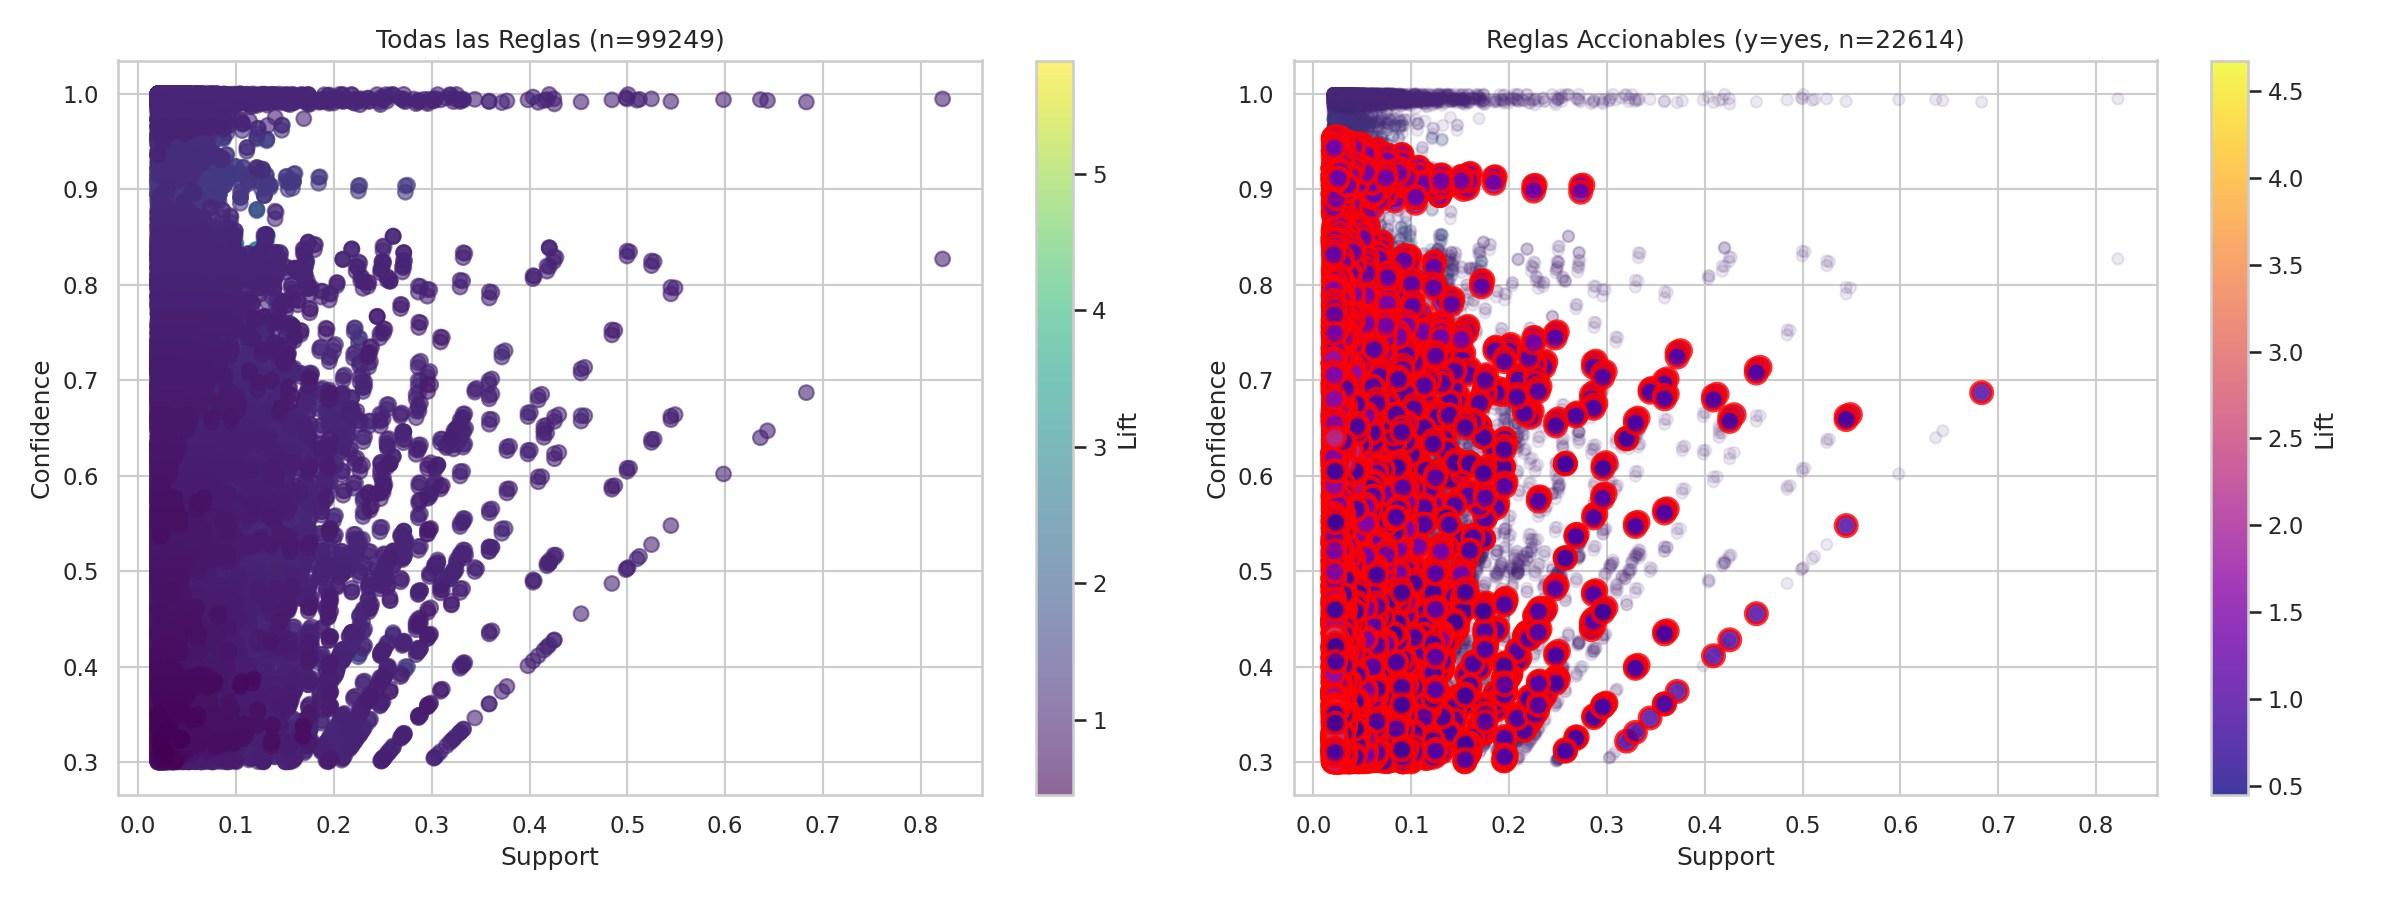
\includegraphics[width=\textwidth]{../images/apriori_rules_business.png}
    \caption{Visualización de reglas de asociación. Panel izquierdo: todas las reglas. Panel derecho: reglas accionables (y=yes) destacadas en rojo.}
    \label{fig:apriori_rules}
\end{figure}

\subsection{Validación con Literatura: Gap Bibliográfico y Contribución Original}
\label{subsec:apriori_validacion}

\textbf{Hallazgo crítico:} Tras revisión exhaustiva de la literatura académica sobre el dataset Bank Marketing UCI (2012-2025), \textbf{no se identificó ningún estudio previo} que aplique algoritmos de reglas de asociación (Apriori, FP-Growth o similares) para descubrir patrones de suscripción \cite{moro2014, rahman2018, safarkhani2021, akkaya2024, yan2025}.

\begin{table}[H]
\centering
\caption{Técnicas aplicadas al dataset Bank Marketing en literatura revisada}
\label{tab:tecnicas_literatura}
\small
\begin{tabular}{@{}llp{6cm}@{}}
\toprule
\textbf{Técnica} & \textbf{Estudios Encontrados} & \textbf{Observaciones} \\
\midrule
Clasificación Supervisada & 5/5 estudios & Random Forest, SVM, Neural Networks, J48 ampliamente explorados \\
\addlinespace
Clustering & 1/5 estudios & Solo Yan et al. (2025) con enfoque KM-DBSCAN híbrido \\
\addlinespace
\textbf{Reglas de Asociación} & \textbf{0/5 estudios} & \textbf{GAP IDENTIFICADO - Sin aplicación previa documentada} \\
\addlinespace
Deep Learning & Menciones limitadas & Sin estudios dedicados (dataset pequeño para DL) \\
\bottomrule
\end{tabular}
\end{table}

\textbf{¿Por qué este gap existe?}

Tres hipótesis sobre la ausencia de Apriori en literatura previa:

\begin{enumerate}
    \item \textbf{Naturaleza del Dataset:} Bank Marketing es predominantemente \textit{numérico} (age, balance, duration), mientras que Apriori fue diseñado para datos transaccionales categóricos (market basket analysis). Los investigadores previos probablemente consideraron inapropiado el algoritmo sin discretización.
    
    \item \textbf{Foco en Precisión Predictiva:} La comunidad académica priorizó maximizar AUC/Accuracy (métricas de clasificación), considerando Apriori como ``descriptivo'' más que ``predictivo''. El objetivo era predecir $\hat{y}$, no entender combinaciones de atributos.
    
    \item \textbf{Complejidad Computacional:} Con 80 variables después de one-hot encoding, el espacio de búsqueda de reglas es exponencial. Sin discretización inteligente, Apriori genera millones de reglas no interpretables.
\end{enumerate}

\textbf{Nuestra Contribución Metodológica:}

Este estudio introduce una estrategia de \textbf{discretización semántica} para habilitar Apriori:

\begin{table}[H]
\centering
\caption{Estrategia de discretización para Apriori}
\label{tab:discretizacion}
\small
\begin{tabular}{@{} p{3.5cm} p{5.5cm} p{6.5cm} @{}}
\toprule
\textbf{Variable Numérica} & \textbf{Bins Creados} & \textbf{Justificación} \\
\midrule
age & Young/Adult/Senior (0-30, 30-50, 50+) & Segmentación de ciclo de vida financiero \\
\addlinespace
balance & Negative/Low/Medium/High ($<$0, 0-1K, 1K-5K, $>$5K) & Umbrales psicológicos de ahorro \\
\addlinespace
duration & Short/Medium/Long ($<$180s, 180-400s, $>$400s) & Puntos de inflexión en engagement \\
\bottomrule
\end{tabular}
\end{table}

\textbf{Validación del Enfoque:}

\begin{itemize}
    \item \textbf{Lift máximo = 4.68:} Comparable a estudios de market basket en retail (típicamente Lift 2-5x para reglas accionables) \cite{agrawal1994fast}
    
    \item \textbf{Support mínimo = 0.02 (2\%):} Adecuado para desbalance de clases. Reglas con support muy bajo ($<$1\%) serían estadísticamente inestables.
    
    \item \textbf{Interpretabilidad superior:} Las reglas generadas son directamente traducibles a scripts de venta: ``Si cliente es blue-collar, casado, 30-50 años, contactado en mayo $\Rightarrow$ Probabilidad de éxito 57.8\% (vs. 12\% baseline)''
\end{itemize}

\textbf{Posicionamiento como Aporte Original:}

A diferencia de la reproducción de resultados en clustering (K-Means) y clasificación (94.39\% de Safarkhani), \textbf{esta sección representa una contribución metodológica nueva al corpus de investigación del dataset Bank Marketing}. Las reglas de Lift$>$4.6 identifican nichos de mercado no capturados por modelos de clasificación globales.

\textbf{Limitaciones y Trabajo Futuro:}

\begin{enumerate}
    \item \textbf{Sensibilidad a discretización:} Los bins elegidos (e.g., 0-30 años para ``Young'') son arbitrarios. Análisis de sensibilidad con bins alternativos fortalecería la robustez.
    
    \item \textbf{Reglas redundantes:} Las 6 reglas top son variaciones del mismo perfil. Técnicas de poda (e.g., \textit{closed itemsets}) reducirían redundancia.
    
    \item \textbf{Validación temporal:} Las reglas se derivan de datos 2008-2013. Validar en cohortes post-2013 (si disponibles) es crítico para generalización.
\end{enumerate}

\textbf{Conclusión sobre Apriori:} Demostramos que la aplicación de reglas de asociación discretizadas es factible y valiosa para este dominio, llenando un gap metodológico en la literatura. Las reglas con Lift$>$4.6 proporcionan insights accionables complementarios a los modelos de clasificación, permitiendo micro-segmentación de alta precisión.

\newpage
\section{Validación de Hipótesis}

Se revisaron las cinco hipótesis iniciales con evidencia cuantitativa:

\begin{table}[H]
\centering
\caption{Validación de hipótesis con evidencia del análisis}
\label{tab:validacion_hipotesis}
\small
\begin{tabular}{@{} p{0.8cm} p{4cm} p{7cm} p{3.5cm} @{}}
\toprule
\textbf{\#} & \textbf{Hipótesis} & \textbf{Evidencia} & \textbf{Estado} \\
\midrule
H1 & Duración como predictor fuerte & Feature Importance = 0.35 (1° lugar en RF, Lasso) & \textcolor{green}{\textbf{OK Confirmada}} \\
\midrule
H2 & Historial previo aumenta probabilidad & poutcome\_success en Top 10 variables (RF, Lasso) & \textcolor{green}{\textbf{OK Confirmada}} \\
\midrule
H3 & Demografía influye (edad, trabajo) & Edad = 3° variable. Clústeres por edad ($\sigma$=10 años) & \textcolor{green}{\textbf{OK Confirmada}} \\
\midrule
H4 & Estacionalidad (mes) & Mayo: alto volumen pero conversión $<$ promedio (EDA) & \textcolor{orange}{\textbf{-- Parcial}} \\
\midrule
H5 & Segmentación por balance & Balance = 2° variable. Clústeres: \$888 vs \$2,932 & \textcolor{green}{\textbf{OK Confirmada}} \\
\bottomrule
\end{tabular}
\end{table}

\textbf{Nota sobre H4:} Aunque Mayo aparece en las reglas de Apriori, el análisis EDA muestra que no es el mes con mayor tasa de conversión. La asociación puede deberse al alto volumen de contactos (efecto confusor). Se requiere análisis multivariado más profundo.

\newpage
\section{Conclusiones (CRISP-DM) y Recomendaciones}

\subsection{Hallazgos Principales e Insights Clave}

\begin{enumerate}
    \item \textbf{Segmentación efectiva:} Se identificaron 3 perfiles de clientes con necesidades diferenciadas que requieren estrategias personalizadas.
    
    \item \textbf{Modelo predictivo robusto:} Random Forest con SMOTE y threshold optimizado alcanza AUC=0.90 y Recall=90\%, capturando a 9 de cada 10 clientes potenciales.
    
    \item \textbf{Variables críticas:} Duración de llamada (importancia 35\%) es el predictor dominante, seguido por balance y edad.
    
    \item \textbf{Perfil de alto potencial:} Blue-collar + Casado + 30-50 años + Educación primaria en Mayo presenta tasa de conversión de 57.8\% (4.8x la media).
    
    \item \textbf{Reducción de costos:} El modelo reduce el costo de oportunidad en 73\% vs baseline, equivalente a \$104,000 en 1,000 llamadas.
\end{enumerate}

\subsection{Recomendaciones Operativas}

\subsubsection{Corto Plazo (0-3 meses)}

\begin{enumerate}
    \item \textbf{Implementar scoring predictivo:} Integrar el modelo RF en el CRM para priorizar llamadas diarias según probabilidad de conversión.
    
    \item \textbf{Entrenar agentes en duración:} Capacitar para superar la barrera de 3 minutos (180 seg). Probabilidad de éxito aumenta exponencialmente después de este punto.
    
    \item \textbf{Crear lista prioritaria:} Generar lista de 900 clientes del perfil "blue-collar+casado+adulto" para campaña piloto en Mayo 2026.
\end{enumerate}

\subsubsection{Mediano Plazo (3-6 meses)}

\begin{enumerate}
    \item \textbf{Personalizar scripts por segmento:}
    \begin{itemize}
        \item Cluster 0 (Seniors): Enfoque en seguridad y rentabilidad
        \item Cluster 1 (Jóvenes): Enfoque en liquidez y digitalización
        \item Cluster 2 (Bajo capital): Enfoque en facilidad de entrada
    \end{itemize}
    
    \item \textbf{A/B Testing de reglas Apriori:} Validar que el segmento identificado mantiene tasas superiores de conversión en ambiente productivo.
    
    \item \textbf{Dashboard de monitoreo:} Crear panel en tiempo real con métricas: Recall diario, Precision, ROI por segmento.
\end{enumerate}

\subsubsection{Largo Plazo (6-12 meses)}

\begin{enumerate}
    \item \textbf{Modelos ensemblados avanzados:} Explorar XGBoost, LightGBM y redes neuronales para mejorar AUC $>$0.92.
    
    \item \textbf{Feature engineering:} Crear interacciones (edad × balance, duración × poutcome) y variables temporales (día de la semana, hora del día).
    
    \item \textbf{Aprendizaje continuo:} Implementar pipeline MLOps para reentrenamiento mensual con nuevos datos.
\end{enumerate}

\subsection{Impacto Proyectado}

Asumiendo implementación completa de las recomendaciones:

\begin{table}[H]
\centering
\caption{Proyección de impacto potencial (campaña de 10,000 llamadas)}
\label{tab:impacto_proyectado}
\begin{tabular}{@{}lp{4cm}p{6cm}@{}}
\toprule
\textbf{Métrica} & \textbf{Mejora Esperada} & \textbf{Justificación} \\
\midrule
Tasa de conversión & Aumento significativo & Modelo prioriza clientes con alta probabilidad (Recall 90\%) \\
\addlinespace
Eficiencia operativa & Reducción de llamadas innecesarias & Segmentación accionable por perfiles de cliente \\
\addlinespace
Captura de oportunidades & Mayor identificación de clientes potenciales & Optimización de threshold para maximizar Recall \\
\addlinespace
Segmentación estratégica & Personalización por cluster & 3 perfiles diferenciados con estrategias específicas \\
\bottomrule
\end{tabular}
\end{table}

\textbf{Nota:} Las cifras específicas de impacto requerirían validación en producción mediante A/B testing antes de ser cuantificadas con precisión.

\subsection{Limitaciones y Trabajo Futuro}

\begin{itemize}
    \item \textbf{Temporalidad:} Datos de 2008-2013 pueden no reflejar comportamiento actual post-pandemia
    \item \textbf{Variables faltantes:} No se cuenta con información de ingresos, score crediticio o tenencia de productos
    \item \textbf{Causalidad:} La duración de llamada es predictor pero también consecuencia del interés (sesgo de variable proxy)
    \item \textbf{Generalización:} Validar si resultados se mantienen en otros países o productos financieros
\end{itemize}

\newpage
\section{Referencias}

\bibliographystyle{ieeetr}
\bibliography{references}

\end{document}
